\chapter{Desarrollo y Validación del Clasificador}
\label{cap:clasificador}

Este capítulo documenta el diseño, implementación y evaluación experimental del módulo de clasificación automática de quejas del sistema. El objetivo central es determinar si una queja admitida en la Defensoría de los Derechos Politécnicos (DDP) corresponde a una de las categorías previstas en el Artículo 4 del Reglamento de la Defensoría. Para ello se construyó un conjunto de \textit{pipelines} de aprendizaje automático que combinan representaciones semánticas de texto con atributos jurídicos explícitos derivados del propio caso.

% ─────────────────────────────────────────────
\section{Ingeniería de Características}
\label{sec:feature_engineering}
% ─────────────────────────────────────────────

La representación de cada queja ante el clasificador se compone de dos fuentes de información complementarias: una semántica, extraída del texto libre de los hechos, y otra jurídica, derivada del análisis estructurado de cada caso.

\subsection{Atributos Jurídicos Booleanos}
\label{subsec:campos_juridicos}

A partir del Artículo 4 del Reglamento de la DDP se definieron siete atributos booleanos que codifican las condiciones normativas relevantes para clasificar una queja. Cada atributo toma el valor $1$ si la condición se cumple y $0$ en caso contrario:

\begin{table}[H]
\centering
\caption{Atributos jurídicos utilizados como características del clasificador}
\label{tab:campos_juridicos}
\begin{tabularx}{\textwidth}{lL}
\toprule
\textbf{Nombre del campo} & \textbf{Descripción} \\
\midrule
\texttt{es\_conflicto\_laboral\_art4\_I} & Conflicto de naturaleza laboral (Art.~4-I) \\
\texttt{es\_evaluacion\_academica\_pura\_art4\_II} & Evaluación académica sin vulneración de derechos (Art.~4-II) \\
\texttt{hay\_vulneracion\_notoria\_de\_derechos} & Vulneración notoria de derechos en contexto evaluativo \\
\texttt{es\_resolucion\_disciplinaria\_art4\_III} & Resolución disciplinaria (Art.~4-III) \\
\texttt{es\_afectacion\_colectiva\_art4\_IV} & Afectación de carácter colectivo (Art.~4-IV) \\
\texttt{involucra\_oic\_art4\_V} & Involucra al Órgano Interno de Control (Art.~4-V) \\
\texttt{hay\_acto\_u\_omision\_de\_autoridad} & Existencia de acto u omisión de autoridad institucional \\
\bottomrule
\end{tabularx}
\end{table}

La extracción de estos atributos se centraliza en la función \texttt{extraer\_features\_juridicos()}, cuyo núcleo es la conversión tipológica de cada campo a entero binario:

\begin{lstlisting}[language=Python, caption={Extracción de atributos jurídicos}, label={lst:extraer_juridicos}]
for campo in CAMPOS_JURIDICOS:
    valor = row.get(campo, False)
    if isinstance(valor, str):
        valor = valor.lower() == "true"
    fila.append(int(bool(valor)))
\end{lstlisting}

La normalización explícita de cadenas de texto (\texttt{"true"/"false"}) garantiza consistencia independientemente del origen del dato (JSON, base de datos, entrada manual).

\subsection{Factor de Amplificación $\alpha$}
\label{subsec:amplificacion}

Los vectores de texto producidos por los modelos de lenguaje tienen entre 300 y 768 dimensiones. Si los atributos jurídicos se concatenaran sin escalar, quedarían diluidos frente al componente semántico. Para contrarrestar esto, se aplica un factor de amplificación $\alpha = 3.0$ antes de la concatenación:

\begin{equation}
\mathbf{x} = \left[\, \mathbf{e} \;\Big|\; \alpha \cdot \mathbf{j} \,\right]
\label{eq:vector_combinado}
\end{equation}

donde $\mathbf{e} \in \mathbb{R}^{d}$ es el embedding textual, $\mathbf{j} \in \{0,1\}^{7}$ el vector de atributos jurídicos y $\alpha = 3.0$ el factor de amplificación. En código:

\begin{lstlisting}[language=Python, caption={Concatenación ponderada de características}, label={lst:amplificacion}]
embeddings = self.vectorizador_.transform(textos)
features_amplificados = features_juridicos * self.peso_juridico  # alpha = 3.0
return np.hstack([embeddings, features_amplificados])
\end{lstlisting}

El valor $\alpha = 3.0$ fue elegido experimentalmente: valores menores no diferenciaban casos limítrofes y valores superiores a $5.0$ sobreajustaban la predicción a los atributos jurídicos, ignorando matices semánticos del texto.

% ─────────────────────────────────────────────
\section{Arquitectura del Pipeline}
\label{sec:arquitectura_pipeline}
% ─────────────────────────────────────────────

El sistema de clasificación se implementó mediante la interfaz \texttt{Pipeline} de \textit{scikit-learn}, lo que garantiza que cada transformación aprendida en entrenamiento se aplique de forma idéntica en inferencia, eliminando el riesgo de fuga de datos (\textit{data leakage}).\cite{pedregosa2011}

\subsection{Estrategias de Vectorización}
\label{subsec:vectorizacion}

Se evaluaron dos representaciones semánticas independientes para determinar cuál captura mejor las particularidades del lenguaje jurídico en español.

\subsubsection{Vectorización con spaCy (\texttt{es\_core\_news\_lg})}

El modelo \texttt{es\_core\_news\_lg} de spaCy genera vectores de 300 dimensiones por token. \cite{honnibal2020} La representación del documento se obtiene promediando únicamente los tokens con vector y que no sean palabras vacías (\textit{stop words}):

%clearpage

\begin{lstlisting}[language=Python, caption={Vectorizador basado en spaCy}, label={lst:spacy_vec}]
tokens = [tok.vector for tok in doc if tok.has_vector and not tok.is_stop]
vecs.append(np.mean(tokens, axis=0) if tokens else np.zeros(300))
\end{lstlisting}

La carga del modelo se realiza de forma \textit{perezosa} (\textit{lazy loading}) dentro del método \texttt{transform()}, lo que evita errores de serialización al guardar el \textit{pipeline} con \texttt{joblib}.

\subsubsection{Vectorización con Sentence-BERT}

El modelo \texttt{paraphrase-multilingual-mpnet-base-v2} produce embeddings de 768 dimensiones entrenados explícitamente para capturar similitud semántica entre oraciones en múltiples idiomas, incluyendo español.\cite{reimers2019}  A diferencia del promedio de tokens de spaCy, este modelo considera el contexto completo de la oración:

\begin{lstlisting}[language=Python, caption={Vectorizador basado en Sentence-BERT}, label={lst:sbert_vec}]
model = SentenceTransformer("paraphrase-multilingual-mpnet-base-v2")
return model.encode(list(textos), show_progress_bar=False)
\end{lstlisting}

Al igual que el vectorizador de spaCy, la instancia del modelo se crea dentro de \texttt{transform()} para compatibilidad con entornos multiproceso.

\subsection{Transformador Combinado (\texttt{VectorizadorCombinado})}
\label{subsec:vectorizador_combinado}

La clase \texttt{VectorizadorCombinado} actúa como transformador unificado compatible con la interfaz \texttt{BaseEstimator} y \texttt{TransformerMixin} de \textit{scikit-learn}. Recibe como entrada un \texttt{DataFrame} con dos columnas: el texto de los hechos y el vector de atributos jurídicos ya calculado. Su salida es la matriz de características combinadas descrita en la \cref{eq:vector_combinado}.

\clearpage

\begin{figure}[h]
    \centering
    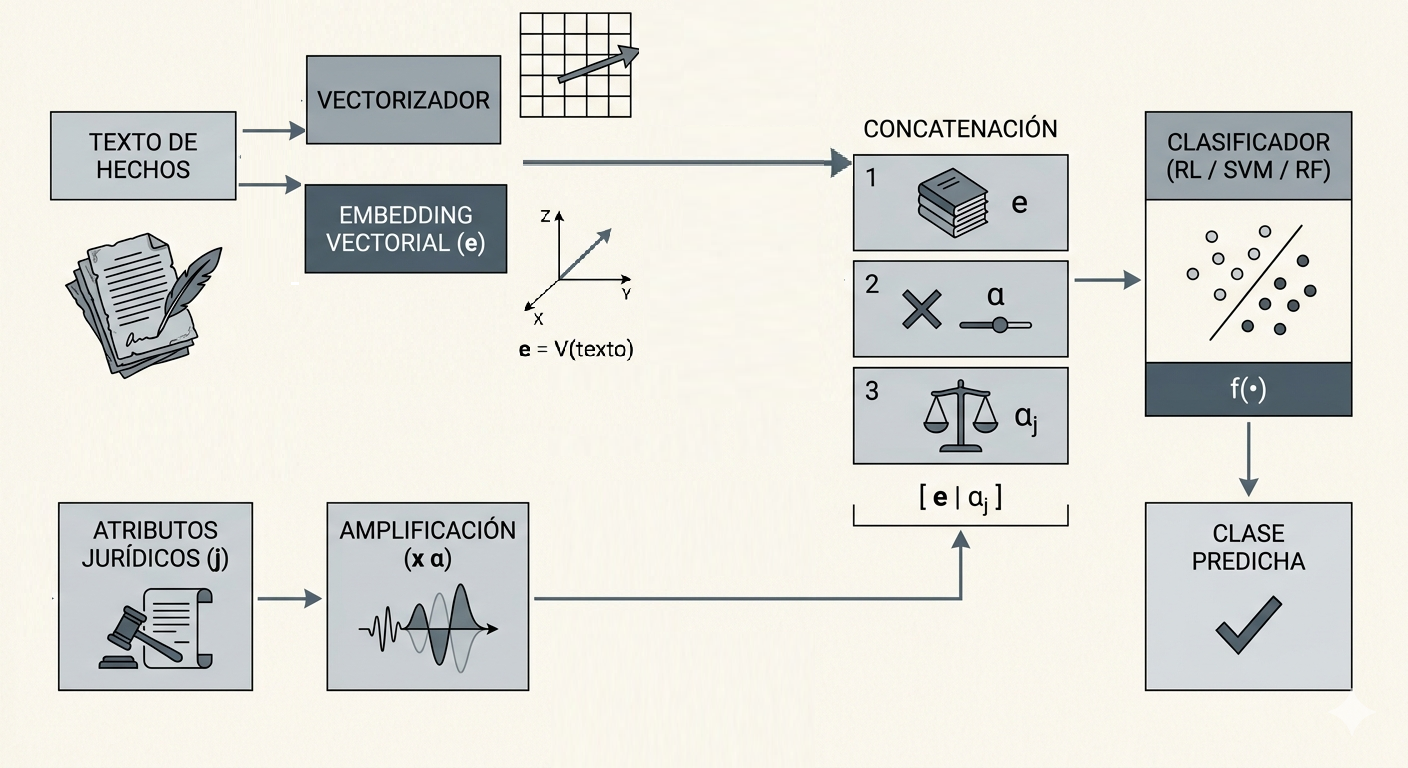
\includegraphics[width=0.9\textwidth]{imagenes/Cap8/ArquitecturaPipeline.png} 
    \caption{Arquitectura del pipeline de clasificaci\'on combinado}
    \label{fig:pipeline}
\end{figure}

La \textbf{Figura \ref{fig:pipeline}} detalla el flujo de datos y la integración de componentes dentro del sistema. El diseño se basa en un enfoque híbrido que procesa simultáneamente información cualitativa y cuantitativa:

\begin{itemize}
    \item \textbf{Extracción de Embeddings ($e$):} El bloque superior representa la transformación del texto libre de los hechos en un vector denso. Dependiendo de la configuración, se utiliza el promedio de vectores de \textit{spaCy} o las representaciones contextuales de \textit{Sentence-BERT}, capturando la semántica narrativa del caso.
    
    \item \textbf{Procesamiento de Atributos Jurídicos ($j$):} Paralelamente, los atributos técnicos identificados en el corpus jurídico son procesados. Se introduce un factor de amplificación ($\alpha$) que permite al investigador ponderar la importancia de estos metadatos frente al texto de los hechos antes de la clasificación.
    
    \item \textbf{Fusión y Clasificación:} El \texttt{VectorizadorCombinado} realiza la concatenación de ambos vectores $[e \mid \alpha \cdot j]$. Este vector resultante, que condensa tanto el contexto lingüístico como el rigor de las variables jurídicas, es entregado al clasificador final para determinar la categoría correspondiente.
\end{itemize}

Esta arquitectura modular asegura que el pipeline sea agnóstico al modelo de lenguaje utilizado, permitiendo intercambiar el vectorizador o el clasificador sin alterar la estructura fundamental del experimento.
\subsection{Construcción Modular del Pipeline}
\label{subsec:pipeline_modular}

La función \texttt{construir\_pipeline\_combinado()} encapsula el ensamblaje del \textit{pipeline}, tomando como parámetros la clase del vectorizador y el clasificador:

\begin{lstlisting}[language=Python, caption={Construcción del pipeline combinado}, label={lst:pipeline_construccion}]
Pipeline([
    ("vectorizador", VectorizadorCombinado(vec_clase, peso_juridico)),
    ("clasificador", copy.deepcopy(clf)),
])
\end{lstlisting}

El uso de \texttt{copy.deepcopy(clf)} es indispensable en el bucle experimental: garantiza que cada combinación reciba una instancia limpia del clasificador, sin estado residual de iteraciones anteriores.

% ─────────────────────────────────────────────
\section{Experimentación y Comparación de Modelos}
\label{sec:experimentacion}
% ─────────────────────────────────────────────

\subsection{Configuración Experimental}
\label{subsec:configuracion_experimental}

Para evaluar cada \textit{pipeline} de manera robusta se adoptó el siguiente protocolo:

\begin{itemize}
    \item \textbf{Partición estratificada 80/20}: preserva la distribución de clases en entrenamiento y prueba, garantizando que clases minoritarias estén representadas en ambos subconjuntos.
    \item \textbf{Validación cruzada} $k=3$ (\textit{3-fold CV}): estima el desempeño esperado en datos no vistos y detecta sobreajuste comparando el F1 del conjunto de prueba contra el F1 promedio de la validación cruzada.
    \item \textbf{Métrica principal}: F1-score ponderado (\textit{weighted}), adecuado para conjuntos con desequilibrio de clases.
\end{itemize}

El protocolo se implementa en \texttt{evaluar\_pipeline\_combinado()}. La línea clave de la validación cruzada es:

\begin{lstlisting}[language=Python, caption={Validación cruzada del pipeline}, label={lst:cv}]
cv_scores = cross_val_score(pipe, df, y, cv=3, scoring="f1_weighted")
\end{lstlisting}

\begin{observacion}[Nota técnica:]
Al usar \texttt{SentenceBERT} se recomienda \texttt{n\_jobs=1} en \texttt{cross\_val\_score} para evitar colisiones de memoria en entornos multiproceso.
\end{observacion}

El espacio experimental cubre $2$ vectorizadores $\times$ $3$ clasificadores $= 6$ combinaciones, entrenadas y evaluadas de forma automática en la función \texttt{comparar\_todos()}:

\begin{lstlisting}[language=Python, caption={Bucle experimental automático}, label={lst:bucle_experimental}]
for vec_nombre, vec_clase in VECTORIZADORES.items():
    for clf_nombre, clf in CLASIFICADORES.items():
        pipe = construir_pipeline_combinado(vec_clase, clf)
        metricas = evaluar_pipeline_combinado(pipe, df_input, etiquetas)
\end{lstlisting}

\subsection{Resultados Cuantitativos}
\label{subsec:resultados}

La \cref{tab:resultados_comparacion} presenta los resultados de los seis experimentos sobre el corpus de casos de la DDP.

\begin{table}[H]
\centering
\caption{Comparación de modelos de clasificación automática de quejas}
\label{tab:resultados_comparacion}
\begin{tabularx}{\textwidth}{llCCCC}
\toprule
\textbf{Vectorizador} & \textbf{Clasificador} & \textbf{Accuracy} & \textbf{F1 (test)} & \textbf{CV F1 $\mu$} & \textbf{CV F1 $\sigma$} \\
\midrule
spaCy avg  & SVM-RBF       & 1.0000 & 1.0000 & 0.9809 & 0.0164 \\
spaCy avg  & Reg. Logística & 1.0000 & 1.0000 & 0.9809 & 0.0164 \\
spaCy avg  & Random Forest  & 0.9810 & 0.9809 & 0.9216 & 0.0381 \\
\midrule
SBERT      & SVM-RBF       & 1.0000 & 1.0000 & \textbf{1.0000} & \textbf{0.0000} \\
SBERT      & Reg. Logística & 1.0000 & 1.0000 & 1.0000 & 0.0000 \\
SBERT      & Random Forest  & 0.9810 & 0.9809 & 0.9790 & 0.0257 \\
\bottomrule
\end{tabularx}
\end{table}

\subsection{Análisis de Desempeño y Selección del Modelo}
\label{subsec:analisis_desempeno}

Los resultados revelan tres patrones claros:

\textbf{Superioridad de SBERT sobre spaCy.} Si bien ambos vectorizadores alcanzan F1 $= 1.0$ en el conjunto de prueba con SVM y Regresión Logística, SBERT produce validación cruzada perfecta ($\mu = 1.0,\ \sigma = 0.0$), lo que indica que su representación contextual es más discriminativa y estable ante distintas particiones del corpus. spaCy, en cambio, presenta varianza de $\sigma = 0.0164$, reflejo de su dependencia del promedio de vectores de tokens independientes.

\textbf{Random Forest como caso inferior.} En ambos vectorizadores, Random Forest exhibe F1 de validación cruzada entre $0.92$ y $0.98$, con la mayor varianza del experimento ($\sigma = 0.0381$ con spaCy). Esto sugiere que el ensamble de árboles no generaliza tan bien como los clasificadores lineales o de margen máximo cuando el espacio de características ya es semánticamente rico.

\textbf{Modelo seleccionado: SBERT + SVM-RBF.} La combinación \texttt{sentence\_bert\_\_SVM\_RBF} es seleccionada para producción al ser la única con varianza nula en validación cruzada, lo que garantiza comportamiento predecible ante casos nuevos. El kernel RBF del SVM proyecta implícitamente las características a un espacio de dimensión superior, hallando fronteras de decisión no lineales que separan perfectamente las categorías jurídicas.

La \cref{fig:f1_comparacion} resume visualmente el F1 ponderado de validación cruzada para los seis experimentos.

% ── Constantes calculadas a mano (ymin=0.88, escala=12 cm por unidad) ──────────
% F1 - 0.88 * 12:  0.9809->1.2108  0.9216->0.4992  1.0000->1.44  0.9790->1.188
% xpos de cada barra (gap=1.1, bw=0.55): 0.375, 1.475, 2.575, 3.675, 4.775, 5.875
\begin{figure}[H]
\centering
\begin{tikzpicture}
  % ── Ejes ────────────────────────────────────────────────────────────────────
  \draw[gray!60, -{latex}] (-0.1, 0) -- (7.0, 0);
  \draw[gray!60, -{latex}] (0, -0.1) -- (0, 1.85)
        node[above, font=\footnotesize] {F1-CV};

  % ── Líneas de referencia ────────────────────────────────────────────────────
  \draw[dashed, gray!40] (0, 0.24) -- (6.6, 0.24);  % 0.90
  \node[left, font=\tiny, gray] at (0, 0.24) {0.90};
  \draw[dashed, gray!40] (0, 0.84) -- (6.6, 0.84);  % 0.95
  \node[left, font=\tiny, gray] at (0, 0.84) {0.95};
  \draw[dashed, gray!40] (0, 1.44) -- (6.6, 1.44);  % 1.00
  \node[left, font=\tiny, gray] at (0, 1.44) {1.00};

  % ── Barras spaCy (azul claro) ───────────────────────────────────────────────
  % spaCy + SVM  F1=0.9809  h=1.2108
  \fill[azulESCOM!35, draw=azulESCOM] (0.1,0) rectangle (0.65, 1.2108);
  \node[above, font=\tiny] at (0.375, 1.2108) {0.9809};
  \node[below, rotate=35, anchor=north east, font=\scriptsize] at (0.375,0) {spaCy+SVM};

  % spaCy + RegLog  F1=0.9809  h=1.2108
  \fill[azulESCOM!35, draw=azulESCOM] (1.2,0) rectangle (1.75, 1.2108);
  \node[above, font=\tiny] at (1.475, 1.2108) {0.9809};
  \node[below, rotate=35, anchor=north east, font=\scriptsize] at (1.475,0) {spaCy+RL};

  % spaCy + RF  F1=0.9216  h=0.4992
  \fill[azulESCOM!35, draw=azulESCOM] (2.3,0) rectangle (2.85, 0.4992);
  \node[above, font=\tiny] at (2.575, 0.4992) {0.9216};
  \node[below, rotate=35, anchor=north east, font=\scriptsize] at (2.575,0) {spaCy+RF};

  % ── Barras SBERT (azul oscuro) ──────────────────────────────────────────────
  % SBERT + SVM  F1=1.0000  h=1.44
  \fill[azulESCOM!80, draw=azulESCOM] (3.4,0) rectangle (3.95, 1.44);
  \node[above, font=\tiny] at (3.675, 1.44) {1.0000};
  \node[below, rotate=35, anchor=north east, font=\scriptsize] at (3.675,0) {SBERT+SVM};

  % SBERT + RegLog  F1=1.0000  h=1.44
  \fill[azulESCOM!80, draw=azulESCOM] (4.5,0) rectangle (5.05, 1.44);
  \node[above, font=\tiny] at (4.775, 1.44) {1.0000};
  \node[below, rotate=35, anchor=north east, font=\scriptsize] at (4.775,0) {SBERT+RL};

  % SBERT + RF  F1=0.9790  h=1.188
  \fill[azulESCOM!80, draw=azulESCOM] (5.6,0) rectangle (6.15, 1.188);
  \node[above, font=\tiny] at (5.875, 1.188) {0.9790};
  \node[below, rotate=35, anchor=north east, font=\scriptsize] at (5.875,0) {SBERT+RF};

  % ── Leyenda ─────────────────────────────────────────────────────────────────
  \fill[azulESCOM!35, draw=azulESCOM] (0.2, 1.65) rectangle (0.6, 1.80);
  \node[right, font=\tiny] at (0.65, 1.725) {spaCy};
  \fill[azulESCOM!80, draw=azulESCOM] (1.6, 1.65) rectangle (2.0, 1.80);
  \node[right, font=\tiny] at (2.05, 1.725) {SBERT};
\end{tikzpicture}
\caption{F1 ponderado (validaci\'on cruzada $k=3$) por combinaci\'on de modelo}
\label{fig:f1_comparacion}
\end{figure}

% ─────────────────────────────────────────────
\section{Persistencia y Gestión del Mejor Modelo}
\label{sec:persistencia}
% ─────────────────────────────────────────────

\subsection{Serialización con \texttt{joblib}}
\label{subsec:serializacion}

Una vez evaluado, cada \textit{pipeline} se serializa en disco con \texttt{joblib}, que maneja eficientemente objetos NumPy de gran tamaño en comparación con el módulo estándar \texttt{pickle}:

\begin{lstlisting}[language=Python, caption={Serialización del pipeline entrenado}, label={lst:serializacion}]
ruta_pkl = f"modelos/{nombre}.pkl"
joblib.dump(pipe, ruta_pkl)
\end{lstlisting}

Cada archivo se nombra con el patrón \texttt{<vectorizador>\_\_<clasificador>\_\_<timestamp>}, lo que permite trazabilidad temporal de los experimentos y coexistencia de múltiples versiones del modelo en el directorio \texttt{modelos/}.

\subsection{Selección Persistente del Mejor Modelo}
\label{subsec:mejor_modelo}

La función \texttt{guardar\_metricas\_mejor\_modelo()} implementa una política de reemplazo conservadora: el archivo \texttt{mejor\_modelo\_metricas.json} sólo se sobreescribe si el F1 del experimento actual supera al del modelo previamente guardado.

\begin{lstlisting}[language=Python, caption={Política de actualización del mejor modelo}, label={lst:mejor_modelo}]
if nuevo_registro["metricas"]["f1_weighted"] > f1_previo:
    json.dump(nuevo_registro, f, indent=2, ensure_ascii=False)
\end{lstlisting}

Esta decisión de diseño protege contra regresiones accidentales de desempeño cuando se realizan experimentos con conjuntos de datos distintos o hiperparámetros diferentes. El JSON resultante incluye metadatos enriquecidos: clave del experimento, \textit{timestamp}, rutas de artefactos, métricas completas y los campos jurídicos utilizados, suficientes para reproducir o auditar el experimento en el futuro.

% ─────────────────────────────────────────────
\section{Validación del Flujo de Inferencia}
\label{sec:inferencia}
% ─────────────────────────────────────────────

\subsection{Flujo de Predicción}
\label{subsec:flujo_prediccion}

La función \texttt{predecir()} encapsula el flujo completo de inferencia. Carga dinámicamente el mejor modelo disponible, construye el \texttt{DataFrame} de entrada y devuelve la clase predicha:

\begin{lstlisting}[language=Python, caption={Función de predicción con carga dinámica del mejor modelo}, label={lst:prediccion}]
mejor_clave = max(res, key=lambda k: res[k]["f1"])
pipe = joblib.load(res[mejor_clave]["ruta_pkl"])

f_vec = np.array([int(bool(features_juridicos.get(c, False)))
                  for c in CAMPOS_JURIDICOS], dtype=np.float32)
df_pred = pd.DataFrame({"texto": [texto],
                         "features_juridicos": [f_vec]})
return pipe.predict(df_pred)[0]
\end{lstlisting}

Nótese que el parámetro \texttt{features\_juridicos} es opcional: si el usuario no lo proporciona, la función inicializa todos los atributos en \texttt{False}, permitiendo clasificar a partir del texto únicamente. Esto habilita dos modos de operación del microservicio: asistido (con los campos jurídicos capturados por el formulario) y autónomo (sólo texto).

\subsection{Casos de Prueba Funcionales}
\label{subsec:casos_prueba}

Se validó el flujo completo de inferencia sobre casos representativos del corpus, verificando que la predicción es consistente tanto con los atributos jurídicos activos como sin ellos. La \cref{tab:casos_prueba} muestra una selección de casos de prueba y sus resultados.

\begin{table}[H]
\centering
\caption{Casos de prueba funcionales del clasificador}
\label{tab:casos_prueba}
\begin{tabularx}{\textwidth}{Lcc}
\toprule
\textbf{Descripción del caso (resumen)} & \textbf{Clase real} & \textbf{Predicción} \\
\midrule
Docente reporta modificación arbitraria de contrato & Laboral (Art.~4-I) & \cmark \\
Alumno impugna calificación de examen ordinario & Evaluación académica (Art.~4-II) & \cmark \\
Alumno denuncia represalia por queja previa & Vulneración de derechos & \cmark \\
Grupo solicita revisión de plan de estudios & Afectación colectiva (Art.~4-IV) & \cmark \\
Irregularidad en licitación reportada al OIC & OIC (Art.~4-V) & \cmark \\
\bottomrule
\end{tabularx}
\end{table}

\begin{observacion}[Limitación conocida:]
El corpus de entrenamiento es de tamaño reducido, lo que explica los valores F1 de validación perfectos. Se recomienda ampliar el conjunto de datos antes de desplegar el modelo en producción y reevaluar con un protocolo de validación cruzada estratificada $k=5$ para obtener estimaciones más conservadoras del desempeño real.
\end{observacion}

\section{Pruebas}
Para validar la capacidad de generalización del sistema y su utilidad real ante usuarios no familiarizados con la normativa, se realizó una fase de pruebas denominada "Modo Autónomo". En esta etapa, el clasificador procesa las quejas ignorando por completo los atributos jurídicos booleanos (fijándolos todos en valor 0), forzando al sistema a basar su veredicto exclusivamente en la representación semántica del texto
\subsection{Definición del Escenario de Prueba}
Se utilizo un conjunto de 40 datos sintéticos de quejas que contienen casos de competencia e incompetencia a la Defensoría, acorde al artículo 4. Cada queja fue sometida a los 6 modelos para obtener aquel que sin necesidad de los atributos jurídicos, logre clasificar de manera adecuada las quejas.

\subsection{Desempeño del Modelo en Ausencia de Metadatos}
La Tabla \ref{tab:resumen_autonomo} resume el desempeño de los modelos bajo esta condición de estrés (sin ayuda de etiquetas jurídicas).

\begin{table}[h]
\centering
\caption{Exactitud de los modelos en Modo Autónomo (Solo Texto)}
\label{tab:resumen_autonomo}
\begin{tabularx}{0.8\textwidth}{Xcc}
\toprule
\textbf{Modelo de Clasificación} & \textbf{Aciertos (40)} & \textbf{Exactitud} \\
\midrule
\texttt{spacy\_avg + SVM\_RBF}           & 40 & 100.00\% \\
\texttt{spacy\_avg + RegLog}             & 39 & 97.50\% \\
\texttt{spacy\_avg + RandomForest}       & 39 & 97.50\% \\
\texttt{sentence\_bert + RandomForest}   & 40 & 100.00\% \\
\texttt{sentence\_bert + RegLog}         & 20 & 50.00\% \\
\texttt{sentence\_bert + SVM\_RBF}       & 20 & 50.00\%* \\
\bottomrule
\end{tabularx}
\end{table}

\textit{Nota: Se observa que el modelo SBERT + SVM presenta una fuerte dependencia del factor de amplificación $\alpha = 3.0$ para separar las clases cuando el corpus es reducido, esto se muestra en los resultados, y modelos como Spacy + SVM y SBERT + RandomForest muestran menor dependencia hacía la información jurídica.}

\subsection{Análisis de Casos Críticos}
Tras procesar los resultados de los archivos de salida, se seleccionaron ejemplos representativos donde el modelo \textbf{spaCy + SVM} y \textbf{SBERT+ Random Forest} demostró robustez absoluta incluso en ausencia de metadatos.

\begin{table}[h]
\centering
\caption{Muestra de inferencias autónomas exitosas}
\label{tab:casos_autonomo}
\begin{tabularx}{\textwidth}{LccC}
\toprule
\textbf{Descripción de la Queja (Resumen)} & \textbf{Clase Real} & \textbf{Predicción} & \textbf{Correcto} \\
\midrule
Profesor reporta retiro de pago de estímulo por trámites administrativos en la ESIME Zacatenco. & No Comp. & No Comp. & \cmark \\
Alumna denuncia discriminación por apariencia física y trato humillante frente al grupo. & Competente & Competente & \cmark \\
Investigación activa del OIC por irregularidades en papelería de oficina en la ENCB. & No Comp. & No Comp. & \cmark \\
\bottomrule
\end{tabularx}
\end{table}

\begin{observacion}
El la Tabla \ref{tab:resultados_comparacion} observamos que todos los modelos presentaban excelentes resultados después de las pruebas, sin embargo, en aquellas pruebas, se mantenía la existencia de los atributos jurídicos de la Tabla \ref{tab:campos_juridicos}, no obstante, al forzar la predicción unicamente con el texto (Tabla \ref{tab:resumen_autonomo}) observamos la superioirdad de Spacy + SVM RBF y SBERT + Random Forest, siendo estos los únicos capaces de predecir con exactitud todas las quejas puesta a prueba.
\end{observacion}